\documentclass[11pt, oneside]{article}   	% use "amsart" instead of "article" for AMSLaTeX format
\usepackage{geometry}                		% See geometry.pdf to learn the layout options. There are lots.
\geometry{letterpaper}                   		% ... or a4paper or a5paper or ... 
%\geometry{landscape}                		% Activate for rotated page geometry
\usepackage[parfill]{parskip}    			% Activate to begin paragraphs with an empty line rather than an indent
\usepackage{graphicx}				% Use pdf, png, jpg, or eps§ with pdflatex; use eps in DVI mode
								% TeX will automatically convert eps --> pdf in pdflatex		
\usepackage{amssymb}
\usepackage{mathtools}
\usepackage{enumerate}
\usepackage{tikz}

\usetikzlibrary{arrows}

\def\firstcircle{(90:1.75cm) circle (2.5cm)}
\def\secondcircle{(210:1.75cm) circle (2.5cm)}
\def\thirdcircle{(330:1.75cm) circle (2.5cm)}

%SetFonts

%SetFonts


\title{\vspace{-3cm} Mec\'anica de Fluidos (2015966)\\Test Prueba \vspace{-0.7cm}}
\vspace{-1cm}
\author{Alejandro Morales \\ \texttt{lmoralesm@unal.edu.co}}
\date{}							% Activate to display a given date or no date

\begin{document}

\maketitle

\vspace{-1.1cm}
\section*{Pregunta 1}\vspace{-0.3cm}
Enuncie las unidades de \emph{masa}, \emph{longitud} y \emph{temperatura} en:
\begin{itemize}
\item[a.] Sistema Ingles
\item[b.] Sistema internacional
\end{itemize}
	

\section*{Pregunta 2}\vspace{-0.3cm}
Convertir las siguientes unidades:
\begin{itemize}
\item[a.] 60.1 $in$ a $cm$ 
\item[b.] 108 $m$ a $ft$
\item[c.] Aceleraci\'on de la gravedad a $ft/s^2$
\end{itemize}
	
\section*{Pregunta 3}\vspace{-0.3cm}
Un carro de juguete de masa $m=50\ kg$ viaja suavemente hacia abajo sobre un plano inclinado a 30$^o$ de la horizontal. Calcular las componentes en $x$ y $y$ de la de la fuerza neta actuante sobre el carro.
	
\section*{Pregunta 4}\vspace{-0.3cm}
Solucionar los siguientes ejercicios:
\begin{itemize}
\item[a.] $\int 3e^x dx$ 
\item[b.] $\int (3x^2 - \sqrt{5x} +2) dx$
\end{itemize}
	
\section*{Pregunta 5}\vspace{-0.3cm}
Dada el area mostrada en la figura, calcular la localizacion del centroide ($\bar{x}$,$\bar{y}$).
\vspace{-0.2cm}
\begin{center}
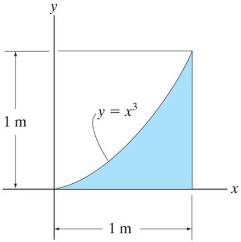
\includegraphics[scale=2.0]{exer5}
\end{center}

	
\end{document} 
